\documentclass[12pt,fleqn]{article}
\setlength{\parindent}{0pt}
\usepackage{graphicx}
\usepackage{listings}
\usepackage[latin5]{inputenc}
\setlength{\parskip}{8pt}
\setlength{\parsep}{0pt}
\setlength{\headsep}{0pt}
\setlength{\topskip}{0pt}
\setlength{\topmargin}{0pt}
\setlength{\topsep}{0pt}
\setlength{\partopsep}{0pt}
\setlength{\mathindent}{0cm}

\begin{document}
Cok Degiskenli Calculus - Ders 12

Zincirleme Kanunu hatirlayalim

\[ \frac{dw}{dt}  = w_x \frac{dx}{dt} + 
w_y \frac{dy}{dt} + 
w_z \frac{dz}{dt}  \]

Bu formul, kismi turevler uzerinden, $w$'daki degisimin $x,y,z$'deki
degisime ne kadar ``hassas'' ne kadar ``bagli'' oldugnu gosteriyor.

Simdi usttekini daha azaltilmis, ozetli (compact, concise) bir formda soyle
yazacagim. 

\[ = \nabla w \cdot  \frac{d\vec{r}}{dt} \]

Gradyan vektoru tum kismi turevlerin bir araya konmus halidir. 

\[ \nabla w = <w_x, w_y, w_z> \]

Tabii ki bunu soyleyince ustteki gradyan'in $x,y,z$'ye bagli oldugunu da
soyluyoruz, mesela $w$'nun belli bir nokta $x,y,z$'da gradyanini
alabilirsiniz, o zaman her degisik $x,y,z$ noktasinda farkli bir vektor
elde edersiniz, ki bu vektorlerin tamamina ileride ``vektor alani (vector
field)'' ismini verecegiz. Devam edelim, 

\[ \frac{d\vec{r}}{dt} = < \frac{dx}{dt}, \frac{dy}{dt}, \frac{dz}{dt} > \]

Yani hiz vektoru (velocity vector) $d\vec{r}/{dt}$ yukaridaki gibi
tanimlidir.

Bugunku amacimiz gradyan vektorunu anlamak, ve nerelerde
kullanabilecegimizi incelemek. Gradyanlari yaklasiksal formullerde
kullanmak mumkundur, vs. Ustte gordugumuz onun notasyonu. 

Gradyanlarin belki de en ``havali'' ozellikleri sudur. 

Teori

Iddia ediyorum ki $\nabla w$ vektoru, $w = \textrm{ bir sabit }$ile elde
edilecek kesit yuzeyine (level surface) her zaman diktir.

Eger fonksiyonumun bir kontur grafigini cizersem

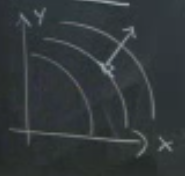
\includegraphics[height=3cm]{12_1.png}

gosterilen noktada hesaplanacak gradyan vektoru o noktadaki kontura
diktir. 

Ornek 1

Lineer bir $w$ kullanalim. 

\[ w = a_1 x + a_2 y + a_3 z \]

Gradyan nedir? Kismi turevleri alalim:

\[ \nabla w = <a_1, a_2, a_3> \]

Konturlari nasil elde ederim? $a_1 x + a_2 y + a_3 z  = c$ ki $c$ bir
sabittir, bu formulu tatmin eden tum $x,y,z$ degerleri bir duzlem
olustururlar. 

Bu duzlemin normalinin nasil alinacagini biliyoruz, katsayilara bakariz,
$<a_1,a_2,a_3>$. Bu vektorun gradyanla ayni ciktigina dikkat, ki normal
vektor de duzleme diktir zaten. Ayni cikmalari mantikli. 

Aslinda bu ornek gradyanin dikligini bir anlamda ispatliyor, cunku duzlem
olmasa bile herhangi bir fonksiyonun birinci yaklasiksalligi bir duzlem
yaratir, o duzlemin normali, gradyani esitligi bizi yine gradyanin
dikligine goturur. Ama bu yeterince ikna edici olmadiysa baska bir ornege
bakabiliriz. 

Ornek 2

\[ w = x^2 + y^2 \]

Bu fonksiyonun kesit seviyeleri, degisik yaricaplara sahip dairelerdir,
$x^2 + y^2 = c$ formulundeki degisik $c$ degerleri bu daireleri tanimlar. 

Gradyan vektoru

\[ \nabla w = <2x, 2y> \]

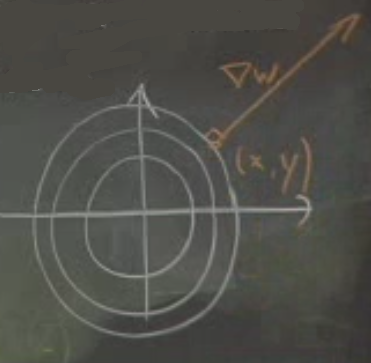
\includegraphics[height=4cm]{12_2.png}

Secilen $x,y$ noktasinda $\nabla w$ gosterilmis. Bu vektorun $x$ ve $y$
eksenlerinde boyunun, basladigi noktaya gore olan $x,y$ degerlerinin
yaklasik iki kati olduguna dikkat, ki bu da $<2x,2y>$ vektoru ile uyumlu. 

Simdi gradyanin niye kesit egrilerine hep dik oldugunu ispatlayalim.

Ispat

Once kesit egrileri ``uzerinde'' hareket eden bir nokta hayal edecegiz. Bu
nokta fonksiyonun sabit oldugu yerlerden geciyor demektir, cunku kontur
uzerinde fonksiyon degeri hep aynidir. 

Egri $\vec{r} = \vec{r}(t)$ hep $w = c$ uzerinde olacak. Resme bakalim,
hayali bir kesit yuzeyi uzerinde bir egri olacak (kirmizi renkli) bu
egrinin uzerinde giden noktanin bir hizi olacak. 

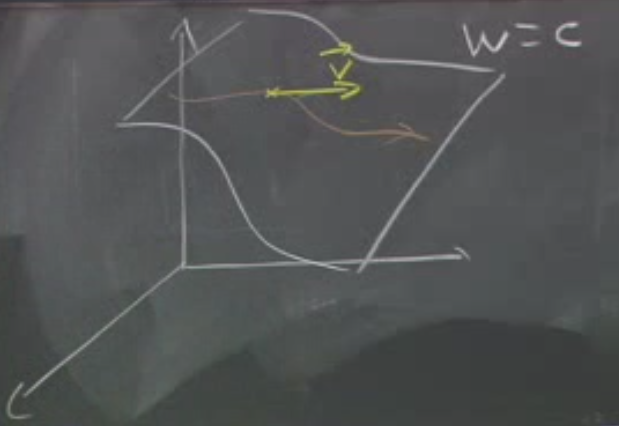
\includegraphics[height=4cm]{12_3.png}

Iddia o ki, 

\[ \vec{r} = \frac{d\vec{r}}{dt} \]

vektoru, kesit $w = c$'ye muhakkak teget olmali, cunku hiz egriye teget, ve
egri kesit icinde. 

Daha baska ne iddia edebiliriz? Zincirleme Kanununu kullanarak 

\[ \frac{dw}{dt} = \nabla w \cdot \frac{d\vec{r}}{dt} \]

esitligini kurabiliriz. 

\[ \frac{dw}{dt} = \nabla w \cdot \vec{v} = 0\]

Sifira esitligin sebebi basta $w = c$ demis olmamiz, o zaman tum kismi
turevler sifirdir ($w$ degerleri sabittir, sabitlerin turevleri sifirdir),
ve $0 \cdot \vec{v} = 0$.

Simdi ters yonden bakalim: iki vektorun noktasal carpimi ne zaman sifir
sonucu verir? Eger vektorler birbirine dik ise. Demek ki $\nabla w \perp
\vec{v}$. Hatta 
iddia ediyorum ki bu diklik $w=c$ uzerindeki her hareket (motion) icin 
gecerlidir. Yani $\vec{v}$, kesit yuzeyine teget olan herhangi bir vektor
olabilir, ustteki diklik hep dogru olacaktir. 




\end{document}
